Her beskrives systemets aktøre. Disse vil blive refereret i de efterfølgende usecase-beskrivelser.

%% !!! Aktør kontekst diagram !!!
%
%\fbox{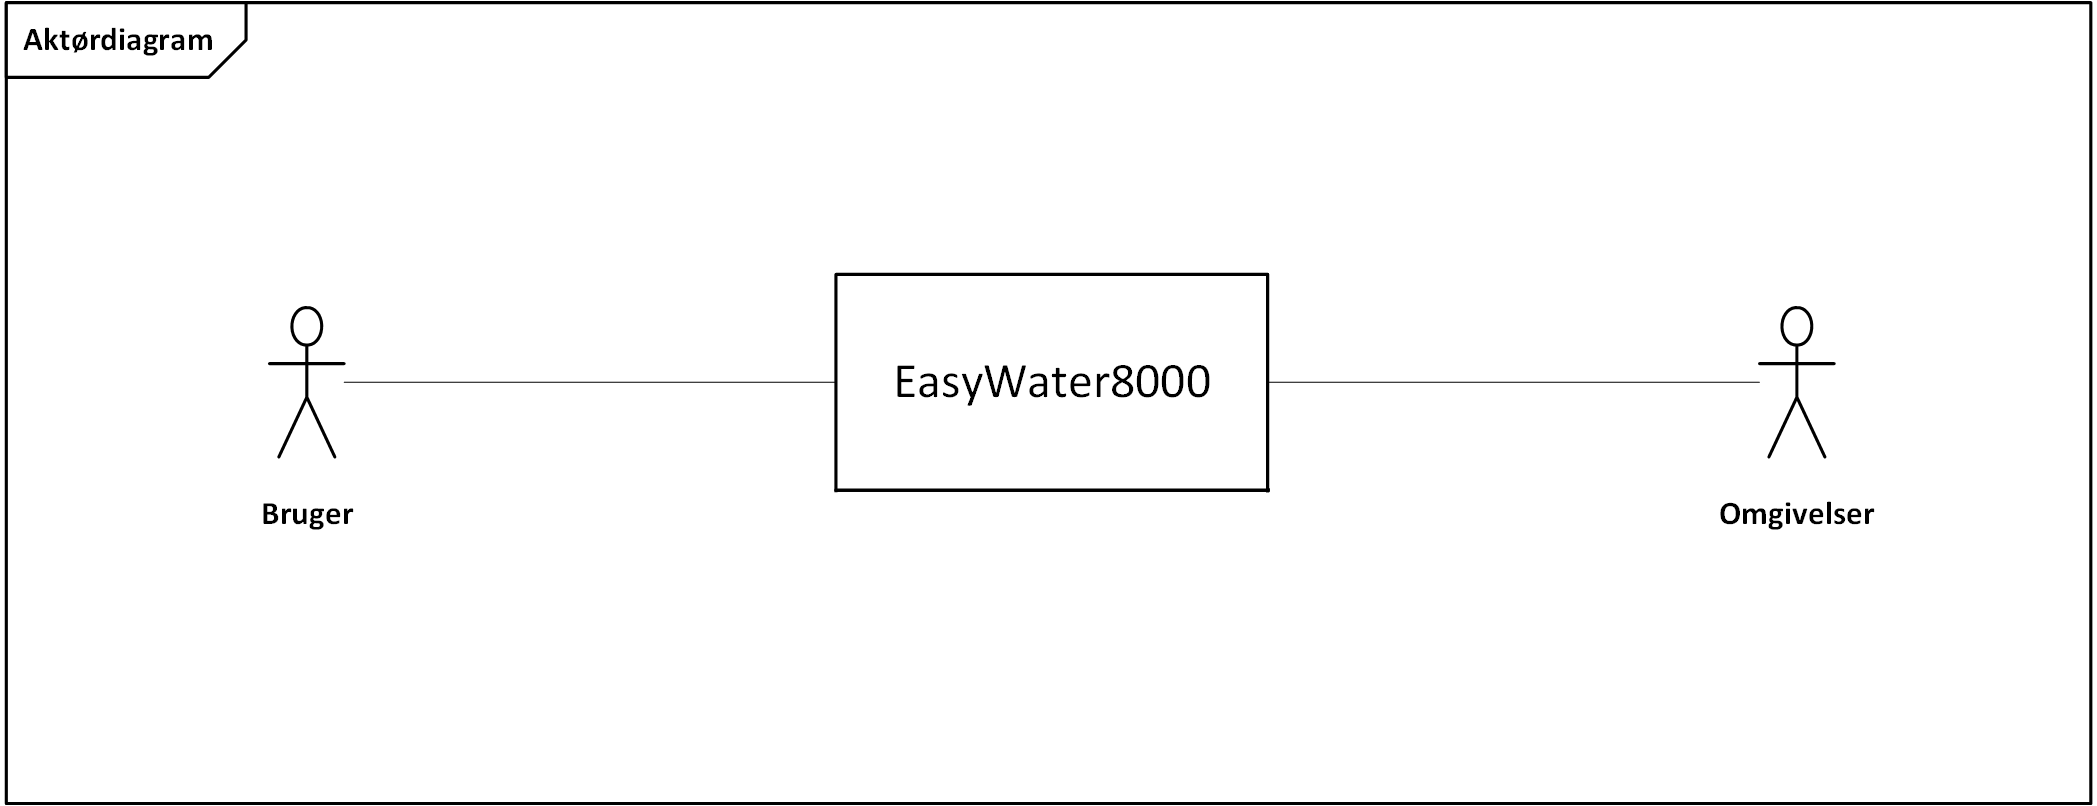
\includegraphics[width=0.9\textwidth]{billeder/diagrammer/Kontekst_Diagram}}
%\caption{Kontekst diagram}
%\label{lab:kontekstdiagram}
%\end{figure}

\begin{table}[!htbp] \centering
	\begin{tabular}{|p{2.5cm}|p{11.5cm}|}
	\hline
		\textbf{Aktør navn} & \textbf{Beskrivelse} \\\hline
		Bruger & Bruger-aktøren vil normalt være greenkeeperen. Det er vedkommende som kontrollere og betjener systemet. (Primær) \\\hline

		Omgivelser & Almene omgivelser, som har indflydelse på systemets sensorer. Det være sig temperatur, fugtighed og bevægelser i områderne omkring systemet. (Sekundær) \\\hline
	\end{tabular}
\end{table}

Ud over de nævnte aktører bruges også navnene på nogle af systemets dele.
